\listfiles
\documentclass[a4paper]{article}

\usepackage{graphicx,amsmath,amssymb,amsfonts}   % Include figure files
\usepackage{dcolumn}    % Align table columns on decimal point
\usepackage{bm}         % bold math
\usepackage{color}
\usepackage{times}
\usepackage{hyperref}
\usepackage{geometry}
\newcommand{\etcs}{\emph{etc. \@} }
\newcommand{\etals}{\emph{et al. \@}}\newcommand{\mb}[1]{\mathbf{#1}}
\newcommand{\ie}{\emph{i.e.\@} }\newcommand{\etc}{\emph{etc.\@} }
\newcommand{\etal}{\emph{et al.\@}}\newcommand{\diffd}{\text{d}}

\hypersetup{backref,
colorlinks=true}

\begin{document}
\title{\texttt{SPECTRA-PKA}}

\maketitle
\section{Introduction}
\texttt{SPECTRA-PKA}~\cite{gilbertmariansublet2015,gilbertsubletNME2016,gilbertsublet2018} is a command-line driven programme for calculating the expected primary knock-on atom (PKA) spectra for a given target nuclide under neutron or charged particle irradiation. NJOY-processed recoil matrices must be provided as the input nuclear data for each nuclide and reaction channel of interest. \texttt{SPECTRA-PKA} will read the nuclear data and collapse the data for each reaction channel in a file with a user-defined energy spectrum of incident particles. \texttt{SPECTRA-PKA} outputs the resulting PKA spectra for each reaction channel read-in, as well as summed PKA distributions for each different recoiling nuclide or element, including both the typically heavy residuals and the secondary-emitted light gas particles. Crucially, \texttt{SPECTRA-PKA} has the ability to process data, in a single run, for a complex material containing many different target species. The user must specify the atomic percentage for each target and the appropriate recoil cross section file, but then \texttt{SPECTRA-PKA} will automatically read-in and process each file and create global average (including as a function of isotope and element) PKA distributions. This feature, in particular, is a significant advancement over what was possible before (such as with \texttt{SPECTER}~\cite{specter} from ANL), where typically PKA distributions were only provided for single elements (and not separated by reaction channel) and based on only one nuclear data library (ENDF/B-V in the case of \texttt{SPECTER}). It allows, for example, the user to investigate the variation in PKA distributions as a function of time under irradiation, where a materials composition may change due to transmutation -- see, for example,~\cite{gilbertsubletNME2016}.

\section{Command line options}
\texttt{SPECTRA-PKA} is executed from the command-line. By default, the programme expects to find an input file called \texttt{specter.input} in the execution folder, but this behaviour can be over-ridden by specifying the name of an input file on the command-line. The input file provides the user with the option to over-ride the default values of the various code words (see below) that \texttt{SPECTRA-PKA} relies upon to control its execution. The input file should be a text file but is largely free from other formatting requirements. Code word values are specified in any order, one per line, via syntax of type:
\begin{center}
\texttt{<code word name>=<code word value>}
\end{center}
A description of each code word and its expected value(s) are given below. An alternative syntax allowing an easier description of a complex alloy (containing multiple target species) is also described.
\section{Code words}
Default values are given in brackets after each code word)
\begin{itemize}


\item \texttt{number{\textunderscore}pka{\textunderscore}files} [\texttt{1}] -- the number of different target species (each with a separate file of recoil cross section input data) to be considered
\item \texttt{pka{\textunderscore}filename} [no default] --- filename(s) of recoil cross section data for each target nuclide. In normal syntax the code word should be followed by \texttt{number{\textunderscore}pka{\textunderscore}files} space-separated (and quoted for complex directory specifications) filenames. The list of filenames may be extended across several consecutive lines. In \texttt{columns} format (see below), one filename will be specified per line.
\item \texttt{flux{\textunderscore}filename} [no default] --- filename containing the incident particle flux spectrum. For compatibility reasons, the format of this file follows closely that used by the \texttt{SPECTER} code. The format is:\\
    \begin{verbatim}
< text description >
<itype> <dummyi> <igroup> <dummyi> <acnm> <time>
<number_groups> <ksail>
< number_groups + 1 energy bin boundaries in MeV>
< number_groups flux values >
    \end{verbatim}
    where \texttt{itype} identifies the type of the flux file. The only type currently supported by \texttt{SPECTRA-PKA} is that where \texttt{itype}\(>1\) -- so that the third line in the file has the \verb|<number_groups><ksail>| format shown above. \texttt{dummyi} are obsolete entries where an integer value is still expected. \texttt{igroup} identifies the units of the subsequent flux values, and an appropriate conversion may be applied according to \verb|flux_norm_type| (see below). In the present code only two choices are accepted: n~s\(^{-1}\) (\texttt{igroup=2}), or n~s\(^{-1}\)~MeV\(^{-1}\) (any other value of \texttt{igroup}), both per unit area. \texttt{acnm} and \texttt{time} were, respectively, used for flux (power) normalization and to obtain the total fluence, but neither of these influence the output produced by \texttt{SPECTRA-PKA}. A \texttt{ksail} value greater than zero indicates that the spectrum file contains error values for the flux in each bin, which are propagated via covariance matrices to the error estimates in the PKA spectrum for each reaction channel (but not to the summed distributions as yet). The flux error vector (\verb|number_groups| values) should immediately follow the \verb|number_groups| flux values.
\item \texttt{flux{\textunderscore}energy{\textunderscore}rescale{\textunderscore}value} [\texttt{1.0}] --- an optional scaling factor to be applied to the boundaries of the input flux spectrum energy bins -- e.g. to convert to the required MeV if not already.

\item \texttt{flux{\textunderscore}rescale{\textunderscore}value} [\texttt{1.0}] --- an optional flux rescale factor that is applied at the time of reading-in the values from the flux file.

\item \texttt{flux{\textunderscore}norm{\textunderscore}type} [\texttt{2}] --- flux normalization control. In the present version of the program, the emphasis is on outputs that are absolute PKAs per second, and so the normalization features are largely obsolete. However, if \verb|flux_norm_type| is 2 then it is assumed that the flux values read-in are per cm\(^2\) and the required conversion to barns (to match the recoil cross sections) is performed. If \verb|flux_norm_type| is 3, then the fluxes used in the subsequent evaluations are exactly those read in from the flux file, with no unit conversion or rescaling. For any other value of \verb|flux_norm_type| the barns conversion is still done, but additionally any unit conversion specified in the flux input file by \texttt{igroup} (see above) is also applied.
\item \texttt{results{\textunderscore}filename} [\texttt{results.out}] --- the string to be used as the name of the file of output the PKA distributions
\item \texttt{results{\textunderscore}stub} [no default] --- a filename stub (beginning) string to be used for both the file of output PKA distributions, and the index file listing the type of each distribution and their location (index) within the main file. If \texttt{results{\textunderscore}stub} is non-empty it overrides any specification within \texttt{results{\textunderscore}filename}. The resulting output files will be named{\begin{center}\texttt{<results{\textunderscore}stub>.out} and \texttt{<results{\textunderscore}stub>.indexes},\end{center}}for the PKA distributions and index file, respectively. If \texttt{results{\textunderscore}stub} is empty the index file will have a default name of \texttt{index{\textunderscore}summary.dat}
\item \texttt{pka{\textunderscore}ratios} [\texttt{1.0} for all targets] --- the weighting factors to be used when combining (summing) results from different targets (each with a separate PKA cross section file). Normally these would be atomic fractions, for example of the naturally occurring isotopes of W, but any non-negative numbers can be used. The user should specify a space-separated list of \texttt{number{\textunderscore}pka{\textunderscore}files} factors. The numbers given need not sum to one -- \texttt{SPECTRA-PKA} will renormalise.


\item \texttt{pka{\textunderscore}filetype} [\texttt{2}] --- an integer specifying the file format of the PKA recoil cross section matrices. The default of 2 is the new style output produced by the UKAEA-modified \texttt{GROUPR} routine of \texttt{NJOY} -- and this is the format distributed to users with the \texttt{SPECTRA-PKA} code. Any other value of \texttt{pka{\textunderscore}filetype} tells the program to expect an old-style format of cross sections -- the format required by \texttt{SPECTER}.


\item \texttt{do{\textunderscore}mtd{\textunderscore}sums} [\texttt{.false.}] --- if true (and if \texttt{pka{\textunderscore}filetype}=2) then produce summed total distributions, for each target species, of \(\alpha\)-particle, proton, inelastic, and scattering (elastic+inelastic) recoils, as well as total distributions of heavy recoils where either \(\alpha\)-particles or protons are produced. The sum distributions are output after the per-reaction-channel distributions of each target.
\item \texttt{do{\textunderscore}ngamma{\textunderscore}estimate} [\texttt{.false.}]  --- if true then estimate the recoils, for each target species, that would results from (\(x,\gamma\)) capture reactions. Recoil cross section matrices for this channel are not output by \texttt{NJOY} and so an approximation is made, using the raw (\(x,\gamma\)) reaction cross section (that must be given in the cross section file of each target) -- see~\cite{gilbertmariansublet2015} for more details. Note that the methodology requires \texttt{SPECTRA-PKA} to know the masses of both the parent (target) and (\(x,\gamma\)) daughter species via \texttt{ngamma{\textunderscore}daughter{\textunderscore}mass} and  \texttt{ngamma{\textunderscore}parent{\textunderscore}mass} -- see below. The (\(x,\gamma\)) recoil distribution is output at the end of the processing of the reaction channels for the current target (but before the sum distributions above).
\item \texttt{ngamma{\textunderscore}parent{\textunderscore}mass} [\texttt{55.934936326} -- \(^{56}\)Fe mass for all targets] --- space-separated list of \texttt{number{\textunderscore}pka{\textunderscore}files} real numbers defining the mass (carbon-12 scale) of each target isotope. Required for calculations of approximate recoil distributions for neutron-capture (\(x,\gamma\)) reactions.
\item \texttt{ngamma{\textunderscore}daughter{\textunderscore}mass} [\texttt{56.935392841} -- \(^{57}\)Fe mass for all targets] =55.934936326{\textunderscore} --- space-separated list of \texttt{number{\textunderscore}pka{\textunderscore}files} real numbers defining the mass (carbon-12 scale) of the daughter nuclide that would result from an (\(x,\gamma\)) reaction on each target. Required for calculations of approximate recoil distributions for neutron-capture (\(x,\gamma\)) reactions.

\item \texttt{parent{\textunderscore}ele} [\texttt{Fe}] --- space-separated list of \texttt{number{\textunderscore}pka{\textunderscore}files} strings defining the element of each target isotope. Used to identify (based on the MT reaction numbers in \texttt{NJOY}) the name an mass number of the daughter for each reaction channel.
\item \texttt{parent{\textunderscore}num}[\texttt{56}] --- space-separated list of \texttt{number{\textunderscore}pka{\textunderscore}files} integers defining the mass number of each target isotope. Used to identify (based on the MT reaction numbers in \texttt{NJOY}) the name an mass number of the daughter for each reaction channel.
\item \texttt{do{\textunderscore}global{\textunderscore}sums} [\texttt{.false.}] --- if true then calculate sum PKA distributions (including as a function of recoiling element and isotope) across all targets using \texttt{pka{\textunderscore}ratios} weighting factors. A final, total, PKA distribution is also produced. The distributions are appended to the PKA output file after the reaction channels of all targets.
\item \texttt{do{\textunderscore}exclude{\textunderscore}light{\textunderscore}from{\textunderscore}total} [\texttt{.true.}] --- if false then include \(\alpha\) and proton recoils in final, total recoil spectra. Not that this should be used with care because such recoils are usually high energy and so including them in the total distribution could significantly alter its profile. The light \(\alpha\) and proton recoils would typically produce a very different kind of damage to a heavy recoil (close to the target mass) of the same energy, and so they should be treated separately.
\item \texttt{do{\textunderscore}exclude{\textunderscore}unknown{\textunderscore}from{\textunderscore}total} [\texttt{.true.}] --- if false then include the PKAs associated with unknown recoil daughters in the total distribution. These ``unknowns'' typically come from (\(n,x\))-like reactions, and it is up to the user to decide if they are important.
\item \texttt{max{\textunderscore}global{\textunderscore}recoils} [\texttt{200}] --- when defining global sums, it is not known in advance how many different recoiling elements or isotopes there will be. In the current version of the code, the array that holds this information is dynamically allocated and so the user must guess an expected upper limit on the number of different recoiling species. 200 is sufficient for most applications.

\item \texttt{energies{\textunderscore}once{\textunderscore}perfile} [\texttt{.false.}] --- if true then for   \texttt{pka{\textunderscore}filetype}=2 the energy bin structure will only be included with the first recoil cross section matrix given in each target file. This overcomes some of the redundancy associated with the default file format, where the input and output bin structure was given with each channel, which came from the legacy format associated with \texttt{SPECTER}. For libraries distributed with \texttt{SPECTRA-PKA}, the new style will be the default, and so \texttt{energies{\textunderscore}once{\textunderscore}perfile=.true.} should be specified (the default may change in future releases).
\item \texttt{do{\textunderscore}tdam} [\texttt{.false.}] --- if true then, for each reaction channel, calculate the equivalent damage-energy bin boundaries associated with each PKA energy bin following the Lindhard-Scharff-Schi{\o}tt~\cite{lindardetal1963a} equations described in~\cite{gilbertsublet2018,robinson1994}. Subsequently, these are used to calculate displacement-energy~\cite{AdrychBrunning2018} and displacements-per-atom (dpa) rates for each bin and the total rates for the reaction channel (see \cite{gilbertsublet2018} for more details). \texttt{SPECTRA-PKA} will also propagate the displacement-energy and dpa rates onto the global sums if \texttt{do{\textunderscore}globals} is also true.
\item \texttt{assumed{\textunderscore}ed} [\texttt{40.0}] --- threshold displacement energy (in eV) for the material used for displacements-per-atom (dpa) evaluation via the Norgett-Robinson-Torrens~\cite{norgettetal1975} formula. A single value to be used for the entire execution. Even in a complex alloy, one atomic species will typically dominate, and so the conversion of damage energy to dpa should use a single value, which could be an average over the major elemental constituents. For example, the typical value for a material dominated by elements such as Fe and its neighbours in the periodic table is 40~eV, and is the default in \texttt{SPECTRA-PKA} (and in many other codes).
\item \texttt{incident{\textunderscore}particle} [\texttt{n}] --- specification of incident particle type. So far, can only be \texttt{n} for neutrons or \texttt{p} for protons. Doesn't alter the results for an individual channel, but is required (for the result to be correct) to identify the daughter product from each reaction, and hence to perform the correct summing by isotope/element/reaction (if \texttt{do{\textunderscore}globals} is true).
\item \texttt{num{\textunderscore}columns} [\texttt{1}] --- the number of different columns (i.e. code words) to be specified in the \texttt{columns} format -- see below
\item \texttt{columns} [no default - specified as required] --- allows specification of input values for the different target species in a column format. Immediately after the code word (after the \texttt{=}) should be a string of space-separated code words, with a number of entries equal to \texttt{num{\textunderscore}columns}. The next \texttt{number{\textunderscore}pka{\textunderscore}files} rows of the input file should specify the values of each code word for each target species to be considered in the execution. Allowed code words in the \texttt{columns} format are\\ \texttt{pka{\textunderscore}filename},\\\texttt{pka{\textunderscore}ratios},\\ \texttt{parent{\textunderscore}ele},\\\texttt{parent{\textunderscore}num},\\ \texttt{ngamma{\textunderscore}parent{\textunderscore}mass},\\ \texttt{ngamma{\textunderscore}daughter{\textunderscore}mass}\\
    A typical use of the \texttt{columns} format, for the 5 naturally occurring isotopes of Zr, and showing all allowable code words in the format, is given below:
\end{itemize}


%\newgeometry{total={8in,10.5in},top=0.55in,headsep=2pt,headheight=0.9in,footskip=0in,
%marginparwidth=0pt,left=0.7cm,centering}	
{\footnotesize
\begin{verbatim}
num_columns=6
columns= pka_filename pka_ratios parent_ele parent_num ngamma_parent_mass ngamma_daughter_mass
"Zr090s.asc" 0.51450000 Zr 90 89.904697659 90.905639587
"Zr091s.asc" 0.11220000 Zr 91 90.905639587 91.905034675
"Zr092s.asc" 0.17150000 Zr 92 91.905034675 92.906469947
"Zr094s.asc" 0.17380000 Zr 94 93.906310828 94.908038530
"Zr096s.asc" 0.02800000 Zr 96 95.908271433 96.910951206
\end{verbatim}}

%\restoregeometry


\section{Input PKA data download}

SPECTRA-PKA uses NJOY-generated recoil cross section matrices. The output files required from NJOY are non-standard and are produced by a slightly modified version of the GROUPR module within NJOY. An evolving selection of databases produced using various international reaction cross section libraries (for various incident particle types) have been pre-calculated and are available to download as compressed tar archives from \url{https://www.ccfe.ac.uk/FISPACT-II/nuclear_data/PKA/}. These can be used immediately with SPECTRA-PKA, or can be used as a template to guide users who may want to create their own input data files (for example, for libraries not currently included on the download page).



\section{Example calculation}
In the folder containing the distributed executables of \texttt{SPECTRA-PKA} there is a ``test'' folder to get the user started. The folder contains the necessary input files to evaluate the PKA distributions of pure zirconium (Zr) in a typical PWR fission spectrum. To run the test navigate to the test folder and then, on the command line, type:
\begin{verbatim}
<location of SPECTRA-PKA>SPECTRA_PKA ZR.in
\end{verbatim}
Here \texttt{<location of SPECTRA-PKA>} is the folder containing the \texttt{SPECTRA-PKA} executable. The \texttt{ZR.in} is:
{\footnotesize
\begin{verbatim}
flux_filename="fluxes_specter.dat"
results_stub="ZR"
num_columns=6
columns= pka_filename pka_ratios parent_ele parent_num ngamma_parent_mass ngamma_daughter_mass
"<PKA data folder>Zr090s.asc" 0.51450000 Zr 90 89.904697659 90.905639587
"<PKA data folder>Zr091s.asc" 0.11220000 Zr 91 90.905639587 91.905034675
"<PKA data folder>Zr092s.asc" 0.17150000 Zr 92 91.905034675 92.906469947
"<PKA data folder>Zr094s.asc" 0.17380000 Zr 94 93.906310828 94.908038530
"<PKA data folder>Zr096s.asc" 0.02800000 Zr 96 95.908271433 96.910951206
flux_norm_type=2
pka_filetype=2
do_mtd_sums=.true.
do_ngamma_estimate=.t.
do_global_sums=.t.
do_exclude_light_from_total=.t.
number_pka_files=5
flux_rescale_value=3.25e14
max_global_recoils=400
energies_once_perfile=.t.
do_tdam=.t.
assumed_ed=40.0
\end{verbatim}}
Note that in the test folder \texttt{<PKA data folder>} in the above has been replaced by the appropriate directory path for the default hierarchy of the \texttt{FISPACT-II} system. The user should tailor this file as necessary to their own system configuration before running the test.

The test folder also has an ``example\verb|_|results'' folder containing the .out and .indexes files that should be produced from a successful execution of the test. The ``plot\verb|_|example'' folder provides example .plt files for \texttt{GNUPLOT} that will produce plots of the summed elemental and isotopic PKA distributions. Users familiar with \texttt{GNUPLOT} will note the use of the \texttt{index} option in each plot command. The index numbers currently used in the .plt files are appropriate for the example results (see \texttt{example\char`_results/ZR.indexes}). \textbf{Important:} Using a different version of the PKA source libraries could result in a different ordering of the results, and so the user should compare the .plt files with the .indexes file from their execution of the test to check that the correct distributions are plotted. The images that should result from this test are given in figure~\ref{pka_graphs}.




\begin{figure}[t]
\hskip-1.5cm
\parbox[b][7cm][t]{0.7\textwidth}{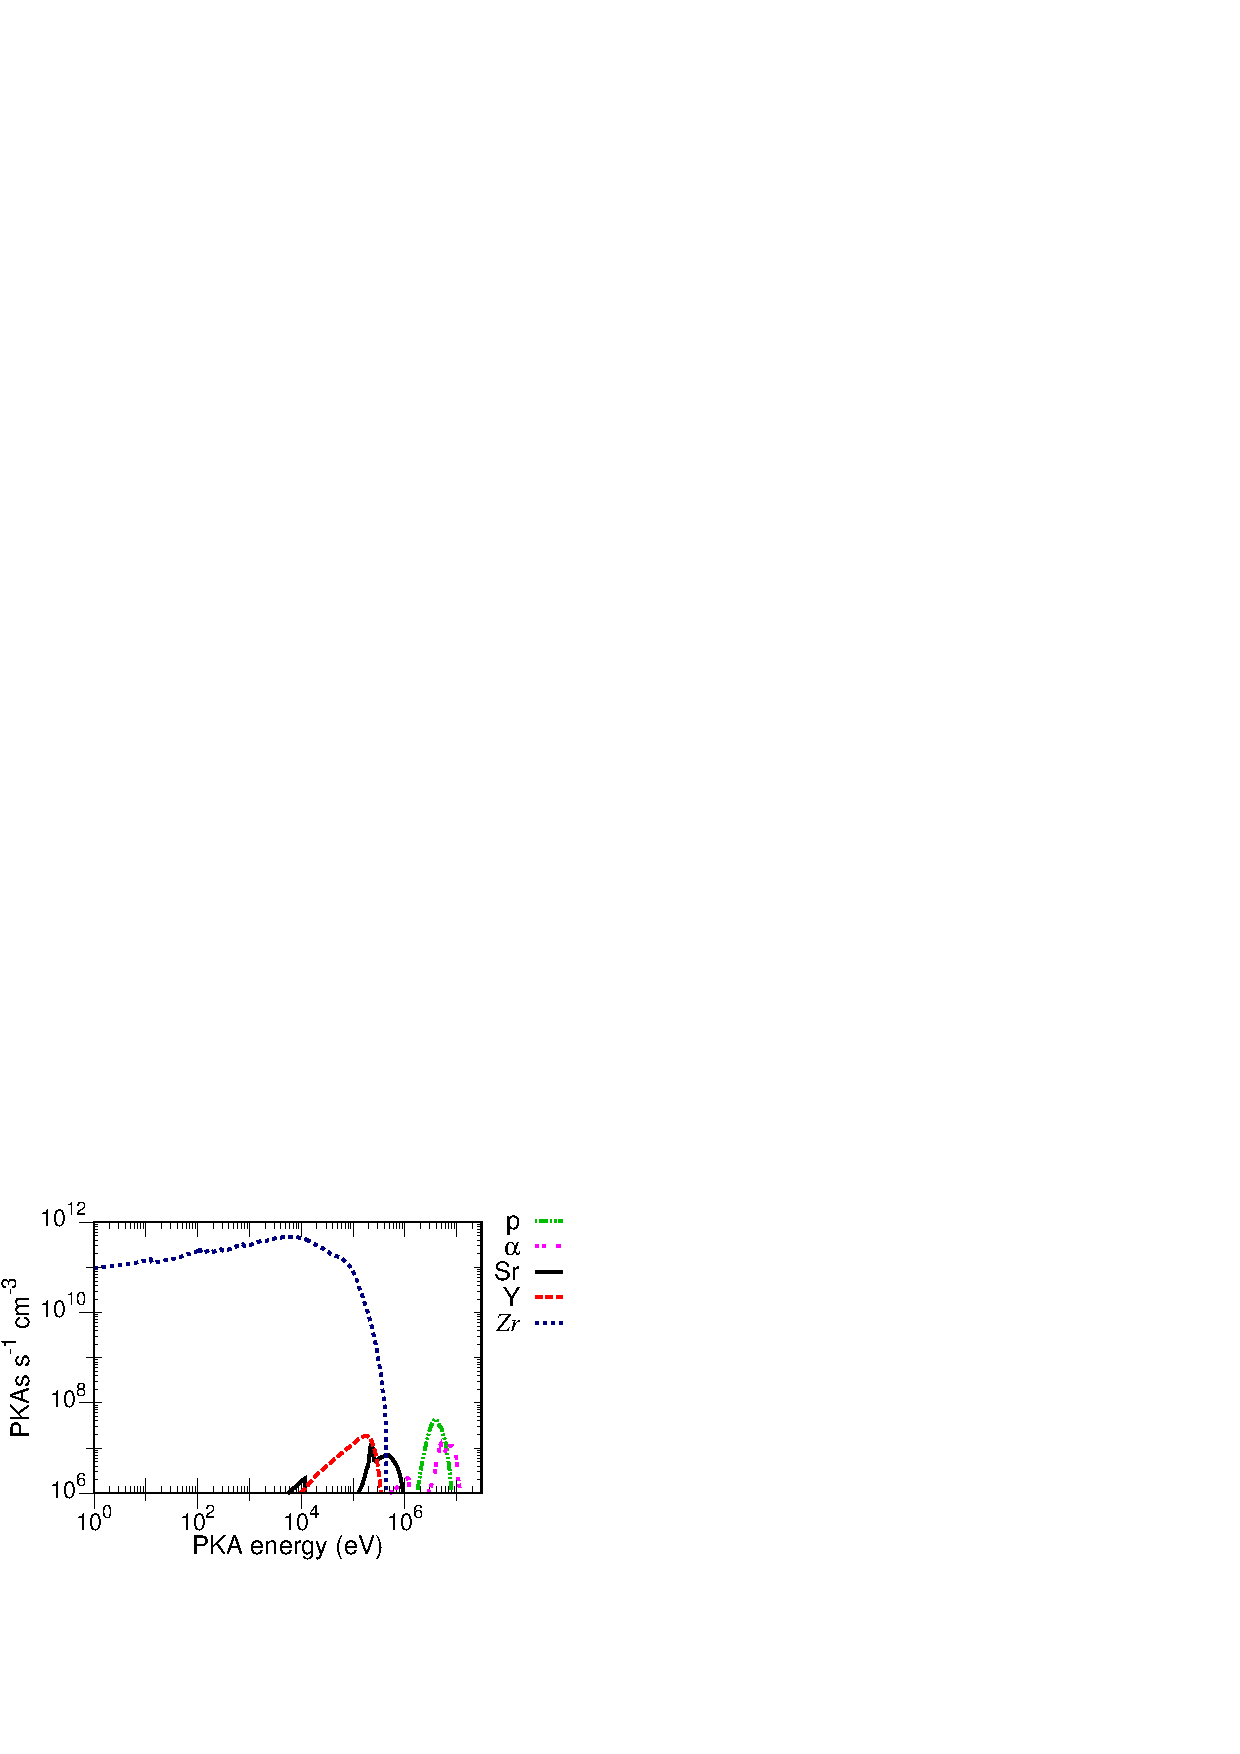
\includegraphics[width=0.7\textwidth]
{ZR_elemental}}%\vskip1cm
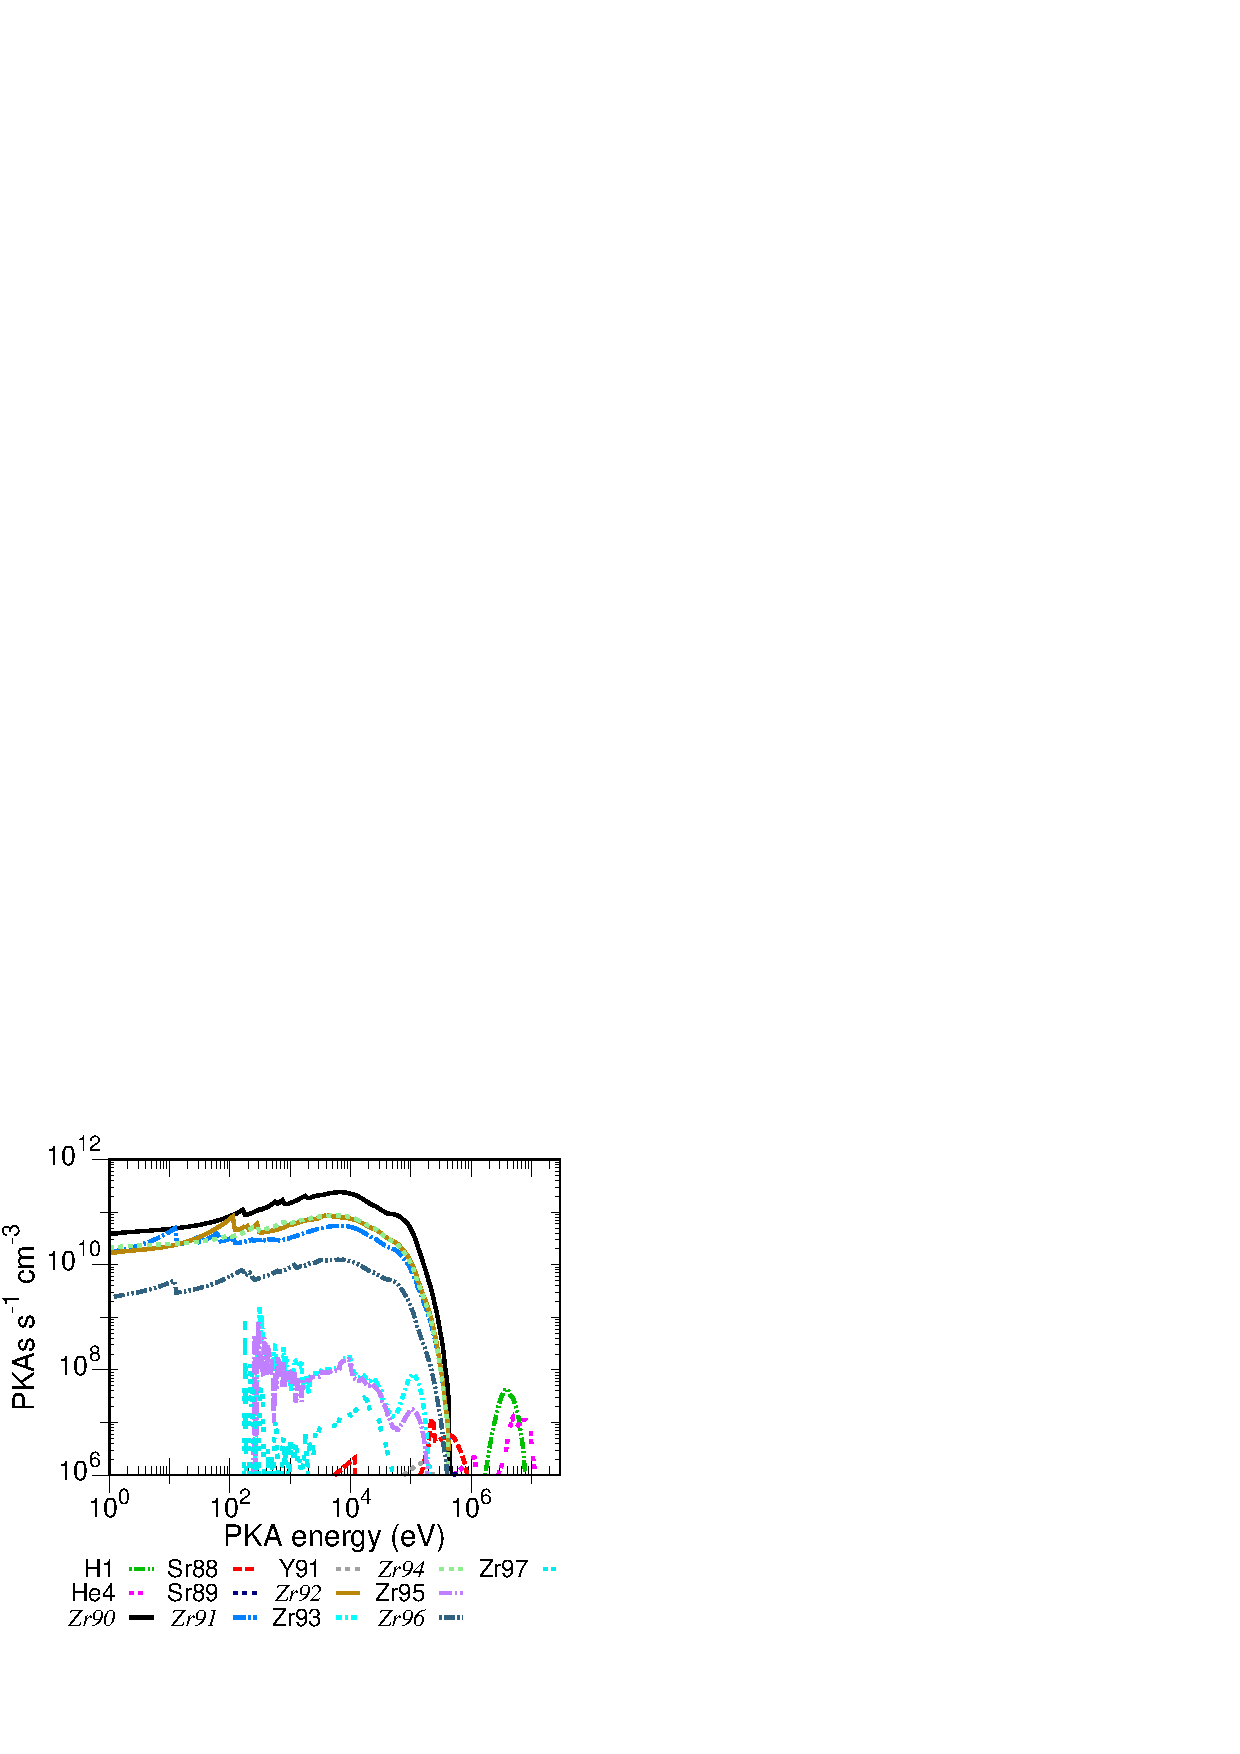
\includegraphics[width=0.5\textwidth]
{ZR_isotope}\\
\vskip-1.0cm
\hskip-0.5cm(a)\hskip7.2cm(b)
\caption{\label{pka_graphs}(a) elemental and (b) isotopic PKA distributions for pure Zr under PWR conditions.}
\end{figure}

\begin{thebibliography}{10}

\bibitem{gilbertmariansublet2015}
M.~R. Gilbert, J.~Marian, and J.~{\relax -Ch}. Sublet, ``Energy spectra of
  primary knock-on atoms under neutron irradiation,'' {\em J. Nucl. Mater},
  vol.~467, pp.~121--134, 2015.
\newblock \url{http://dx.doi.org/10.1016/j.jnucmat.2015.09.023}.

\bibitem{gilbertsubletNME2016}
M.~R. Gilbert and J.-{\relax Ch}. Sublet, ``{{PKA distributions: Contributions
  from transmutation products and from radioactive decay}},'' {\em Nucl. Mater.
  Energy}, vol.~9, pp.~576--580, 2016.
    \newblock \url{http://dx.doi.org/10.1016/j.nme.2016.02.006}.

\bibitem{gilbertsublet2018}
M.~R. Gilbert and J.-{\relax Ch}. Sublet, ``{{Differential dpa calculations with SPECTRA-PKA}},'' {\em J. Nucl. Mater.}, accepted for publication, 2018.

\bibitem{specter}
L.~R. Greenwood and R.~K. Smither,
  ``Specter: Neutron damage calculations for materials
  irradiations'', January 1985. Document Number:
  ANL/FPP/TM-197. SPECTER and SPECOMP are available from the NEA databank.
\newblock \url{http://www.oecd-nea.org/tools/abstract/detail/psr-0263}.



\bibitem{lindardetal1963a}
J.~Lindhard, M.~Scharff, and H.~E. Schi{\o}tt,
  ``{{Range concepts and heavy
  ion ranges (notes on atomic collisions, {II})}},'' {\em Mat. Fys. Medd. Dan. Vid.
  Selsk}, vol.~33~(14), pp.~1--42, 1963.
\newblock\url{https://www.osti.gov/scitech/biblio/4153115}

\bibitem{robinson1994}
M.~T. Robinson, ``{{Basic physics of radiation damage production}},'' {\em J. Nucl. Mater.}, vol.~216, pp.~1--28, 1994.
\newblock 
  \url{https://doi.org/10.1016/0022-3115(94)90003-5}


\bibitem{AdrychBrunning2018}
A.~Adrych-Brunning, M.~R.~Gilbert, J.~{\relax -Ch}. Sublet, A.~Harte, and C.~P.~Race, ``Modelling the interaction of primary irradiation damage and
precipitates: Implications for experimental irradiation of zirconium
alloys,'' {\em J. Nucl. Mater},
  vol.~498, pp.~282--289, 2018.
\newblock \url{https://doi.org/10.1016/j.jnucmat.2017.10.022}.

\bibitem{norgettetal1975}
M.~J. Norgett, M.~T. Robinson, and I.~M. Torrens, ``{{A proposed method of calculating
  displacement dose rates}},'' {\em Nucl. Eng. Des.}, vol.~33, pp.~50--54, 1975.
\newblock \url{https://doi.org/10.1016/0029-5493(75)90035-7}.







\end{thebibliography}

\end{document}
